\section{Design}
En udbredt metode, at udvikle en effektforstærker efter, er LIN 3-stage topologien\fixme{kilde: Jan, mm20}. Efter den topologi opbygges en effektforstærker som en kæde bestående af en differensforstærker efterfulgt af en spændingsforstærker, igen efterfulgt af en strømforstærker. Der er desuden et tilbagekoblingsnetværk også. 

\begin{figure}[h]
\centering
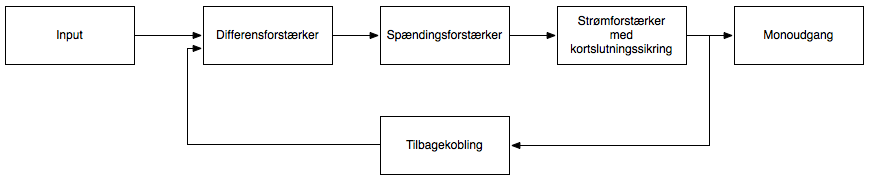
\includegraphics[scale=0.5]{teknisk/effektforstaerker/blokdiagram-effektforstaerker.png}
\caption{Blokdiagram af effektforstærkeren.}
\label{fig:lin_effektforstaerker}
\end{figure}

Som vist på figur \ref{fig:lin_effektforstaerker}, er det ene signal i differensforstærkeren inputtet til effektforstærkeren, mens det andet er en tilbagekobling af outputtet. LIN 3-stage topologien vil blive benyttet i denne designproces, som vil starte bagfra i forhold til opbygningen på figur \ref{fig:lin_effektforstaerker}. 